% Created 2020-05-21 Thu 22:34
% Intended LaTeX compiler: pdflatex
\documentclass[10pt, compress, aspectratio=169, xcolor={table,usenames,dvipsnames}]{beamer}

\usepackage{booktabs}
\mode<beamer>{\usetheme[numbering=fraction, progressbar=none, titleformat=smallcaps, sectionpage=none]{metropolis}}
\usepackage{sourcecodepro}
\usepackage{booktabs}
\usepackage{array}
\usepackage{listings}
\usepackage{caption}
\usepackage{xeCJK}
\usepackage{graphicx}
\usepackage[english]{babel}
\usepackage[scale=2]{ccicons}
\usepackage{hyperref}
\usepackage{relsize}
\usepackage{amsmath}
\usepackage{bm}
\usepackage{wasysym}
\usepackage{ragged2e}
\usepackage{textcomp}
\usepackage{pgfplots}
\usepgfplotslibrary{dateplot}
\definecolor{Base}{HTML}{191F26}
\definecolor{Accent}{HTML}{bb0300}
\setbeamercolor{alerted text}{fg=Accent}
\setbeamercolor{frametitle}{bg=Base}
\setbeamercolor{normal text}{bg=black!2,fg=Base}
\setsansfont[BoldFont={Source Sans Pro Semibold},Numbers={OldStyle}]{Source Sans Pro}
\lstdefinelanguage{Julia}%
{morekeywords={abstract,struct,break,case,catch,const,continue,do,else,elseif,%
end,export,false,for,function,immutable,mutable,using,import,importall,if,in,%
macro,module,quote,return,switch,true,try,catch,type,typealias,%
while,<:,+,-,::,/},%
sensitive=true,%
alsoother={$},%
morecomment=[l]\#,%
morecomment=[n]{\#=}{=\#},%
morestring=[s]{"}{"},%
morestring=[m]{'}{'},%
}[keywords,comments,strings]%
\lstset{ %
backgroundcolor={},
basicstyle=\ttfamily\scriptsize,
breakatwhitespace=true,
breaklines=true,
captionpos=n,
commentstyle=\color{Accent},
extendedchars=true,
frame=n,
keywordstyle=\color{Accent},
language=R,
rulecolor=\color{black},
showspaces=false,
showstringspaces=false,
showtabs=false,
stepnumber=2,
stringstyle=\color{gray},
tabsize=2,
}
\renewcommand*{\UrlFont}{\ttfamily\smaller\relax}
\graphicspath{{../../img/}}
\addtobeamertemplate{block begin}{}{\justifying}
\captionsetup[figure]{labelformat=empty}
\usetheme{default}
\author{ \vspace{-2em} \footnotesize Pedro Bruel \newline \scriptsize \emph{phrb@ime.usp.br}}
\date{\scriptsize May 25th, 2020}
\title{ Introduction to OS-Level Virtualization on Linux}
\hypersetup{
 pdfauthor={ \vspace{-2em} \footnotesize Pedro Bruel \newline \scriptsize \emph{phrb@ime.usp.br}},
 pdftitle={ Introduction to OS-Level Virtualization on Linux},
 pdfkeywords={},
 pdfsubject={},
 pdfcreator={Emacs 26.3 (Org mode 9.2.5)},
 pdflang={English}}
\begin{document}

\maketitle

\section{Introduction}
\label{sec:org6f4ebeb}
\begin{frame}[label={sec:org69f49ad}]{What are Simulation, Emulation, Virtualization?}
\begin{columns}
\begin{column}{0.75\columnwidth}
\only<1-2>{
\begin{center}
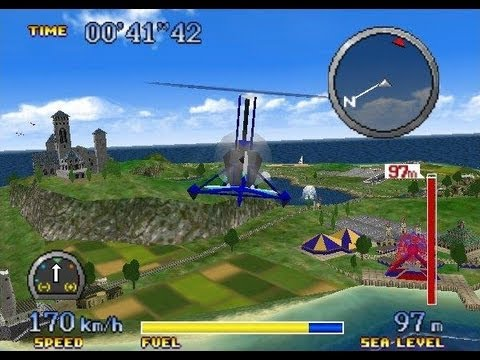
\includegraphics[width=0.9\columnwidth]{../../img/pilotwings64.jpg}
\end{center}
}
\only<3>{
\begin{center}
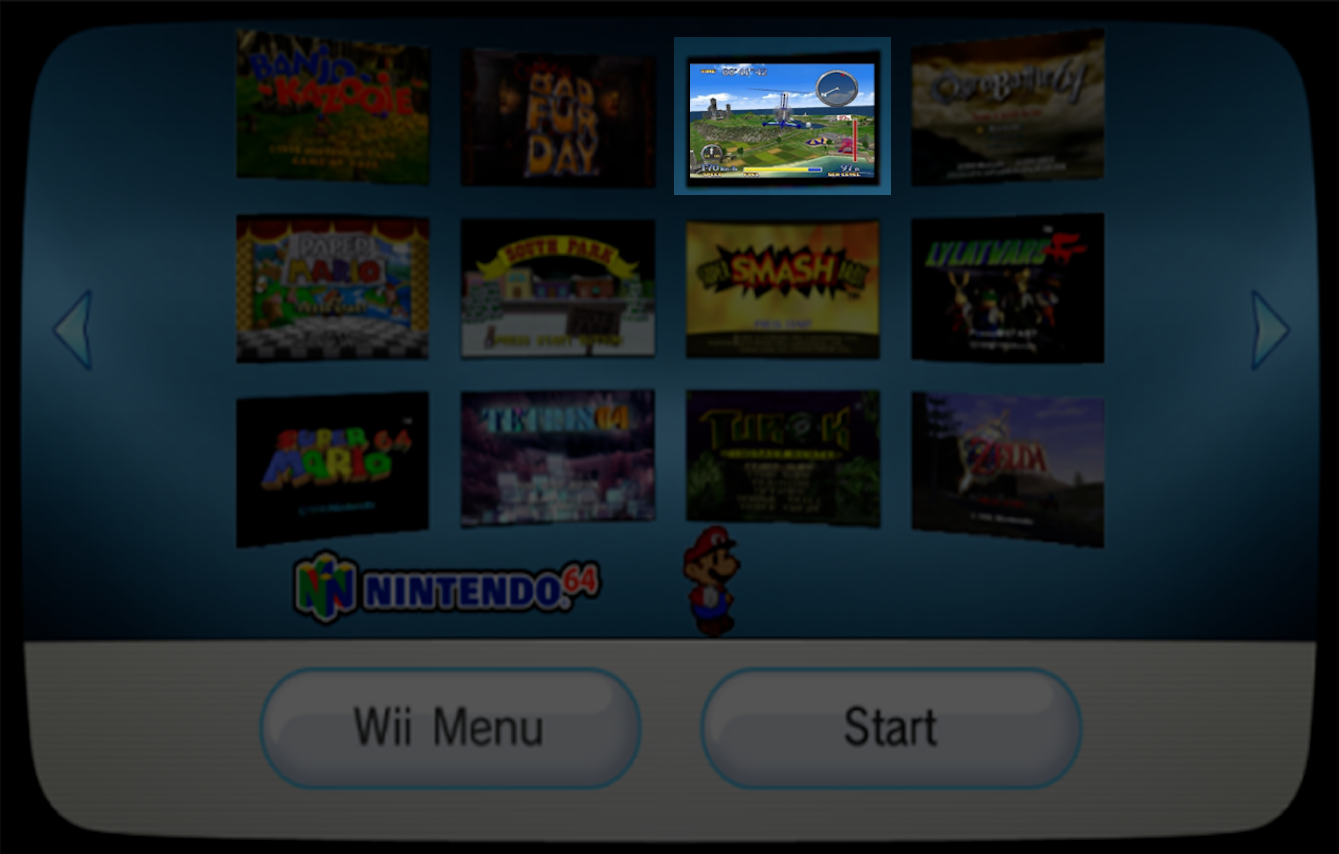
\includegraphics[width=0.9\columnwidth]{../../img/wii_n64.png}
\end{center}
}
\only<4>{
\begin{center}
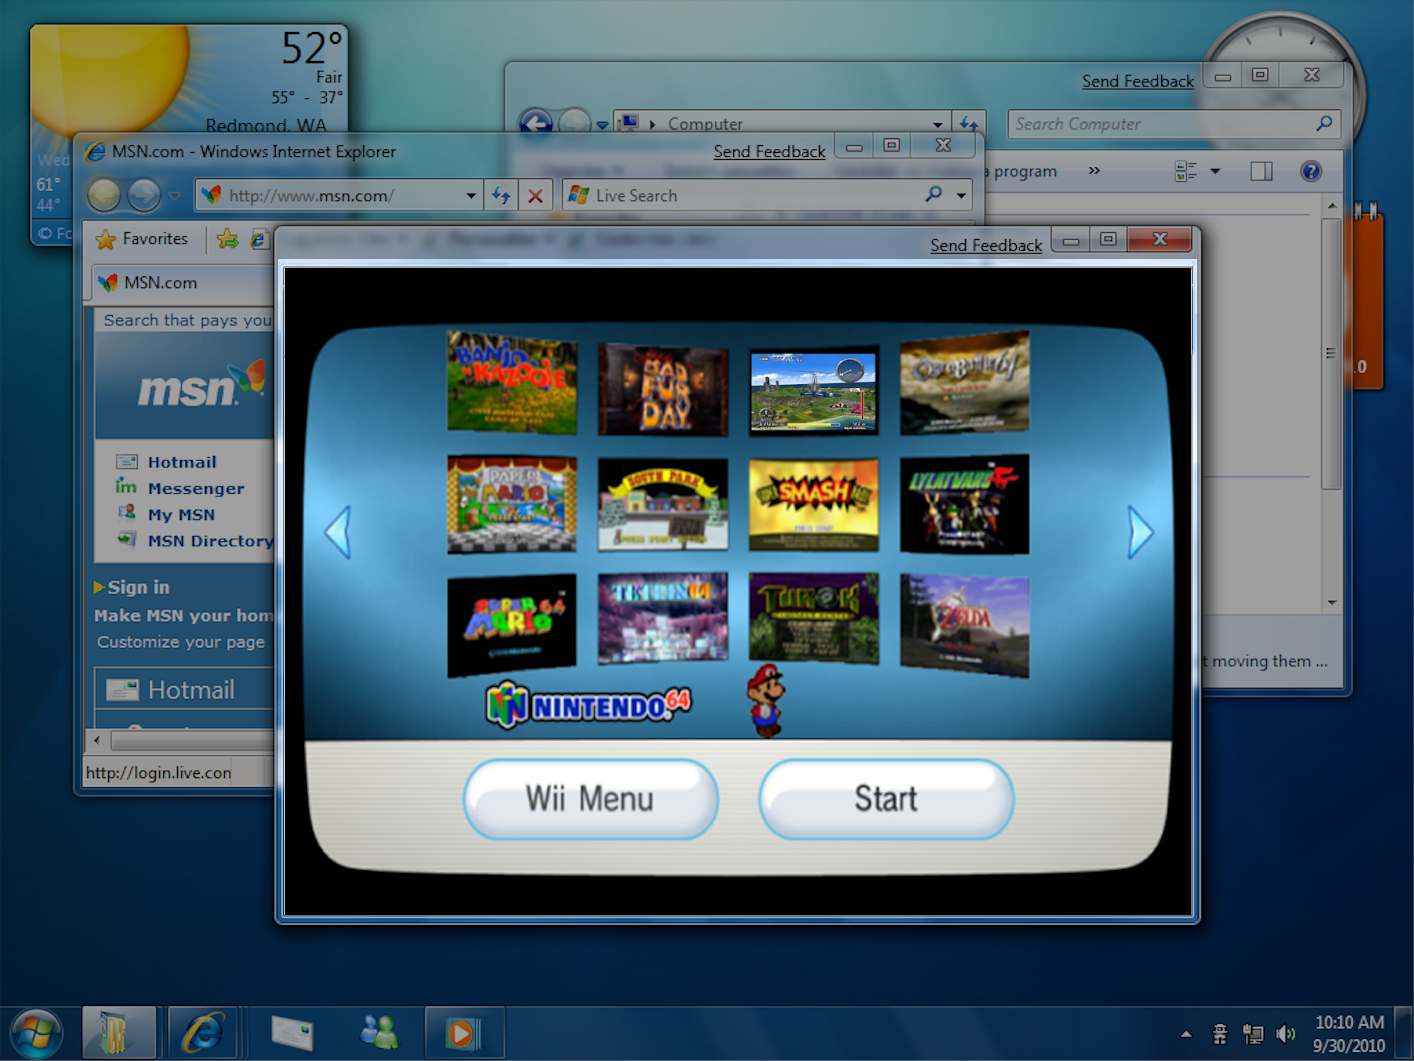
\includegraphics[width=0.9\columnwidth]{../../img/wii_n64_win7.png}
\end{center}
}
\only<5-6>{
\begin{center}
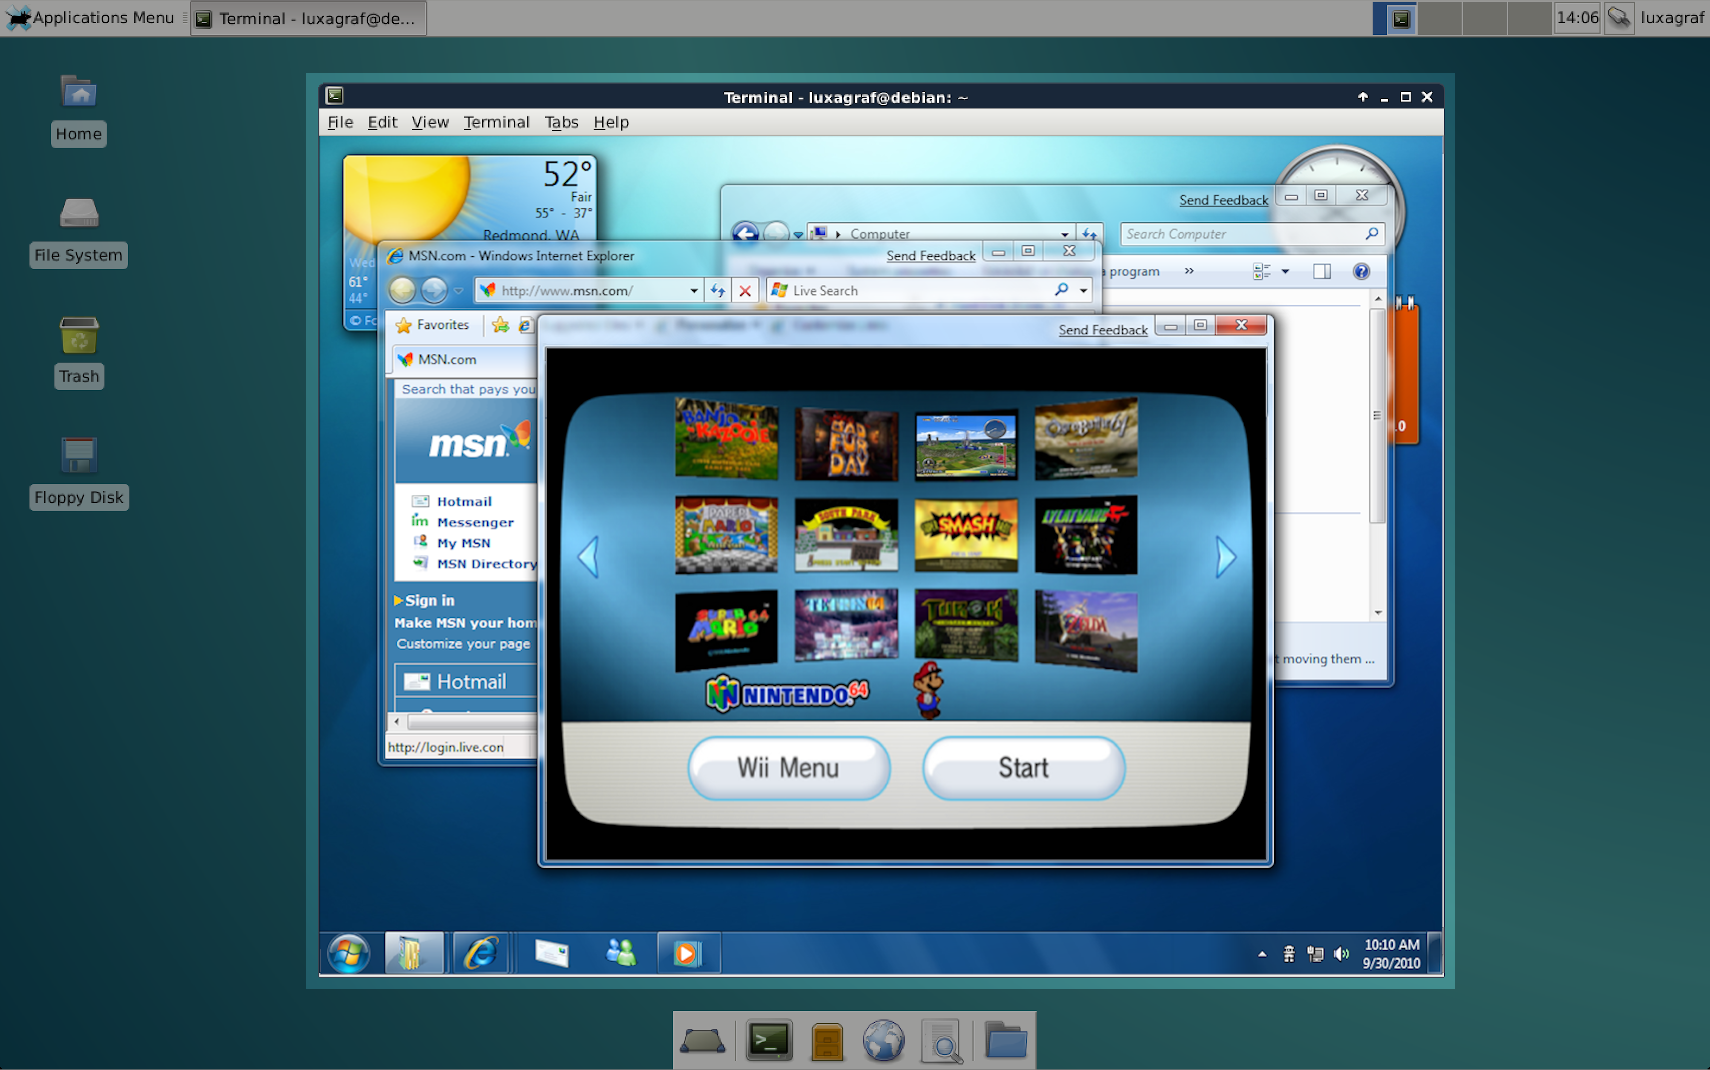
\includegraphics[width=0.9\columnwidth]{../../img/wii_n64_win7_debian.png}
\end{center}
}
\end{column}

\begin{column}{0.25\columnwidth}
\only<1>{
\begin{center}
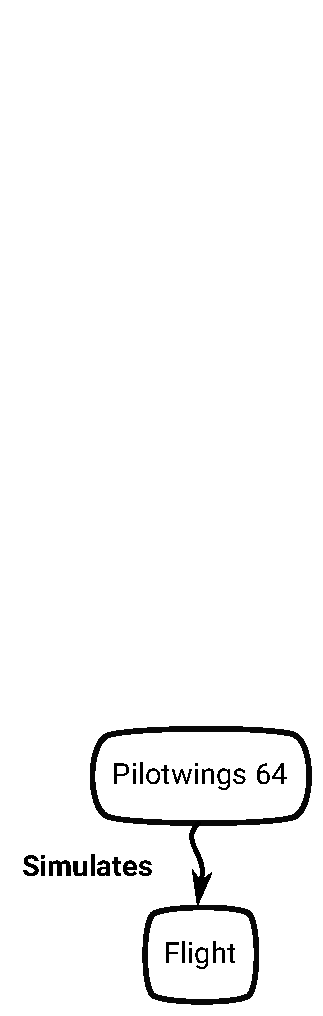
\includegraphics[width=.7\columnwidth]{../../img/pw64_flight.pdf}
\end{center}
}
\only<2>{
\begin{center}
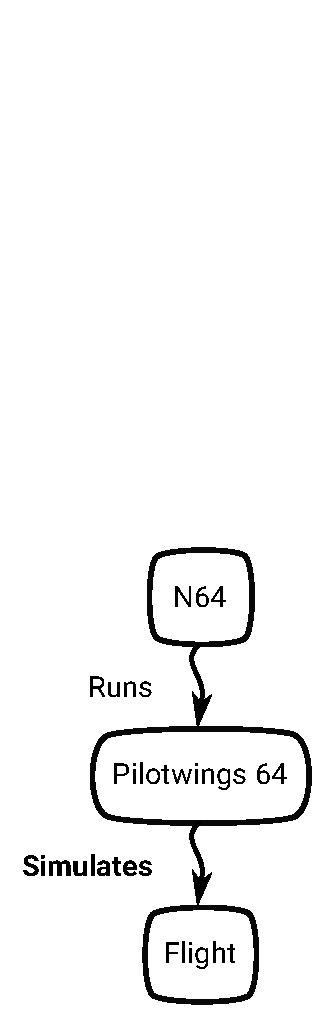
\includegraphics[width=.7\columnwidth]{../../img/n64_pw64_flight.pdf}
\end{center}
}
\only<3>{
\begin{center}
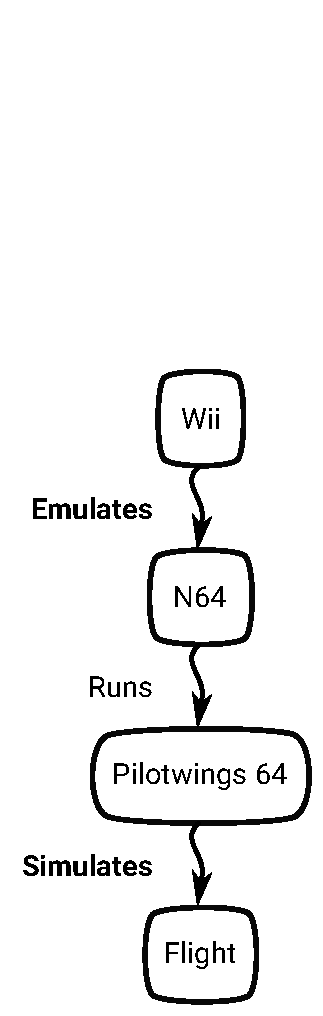
\includegraphics[width=.7\columnwidth]{../../img/wii_n64_pw64_flight.pdf}
\end{center}
}
\only<4>{
\begin{center}
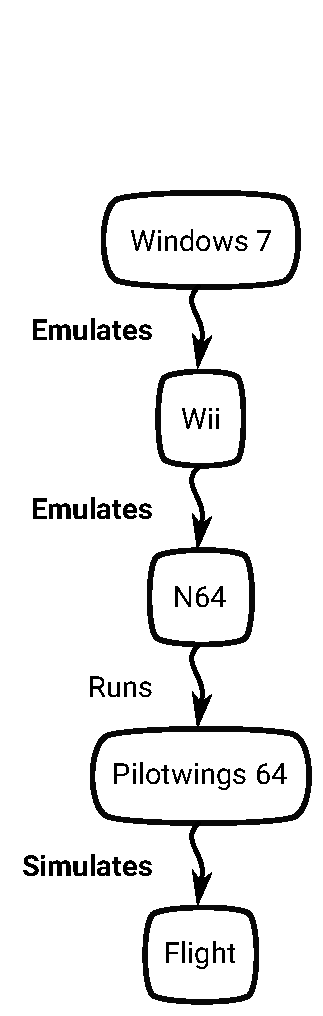
\includegraphics[width=.7\columnwidth]{../../img/win7_wii_n64_pw64_flight.pdf}
\end{center}
}
\only<5>{
\begin{center}
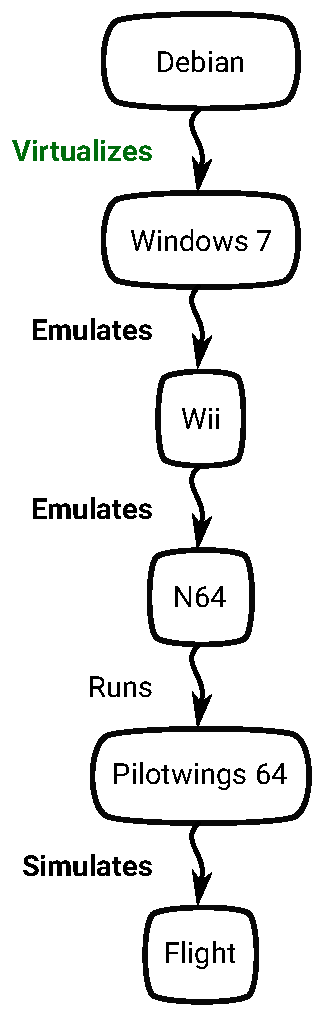
\includegraphics[width=.7\columnwidth]{../../img/debian_win7_wii_n64_pw64_flight.pdf}
\end{center}
}
\only<6>{
\begin{center}
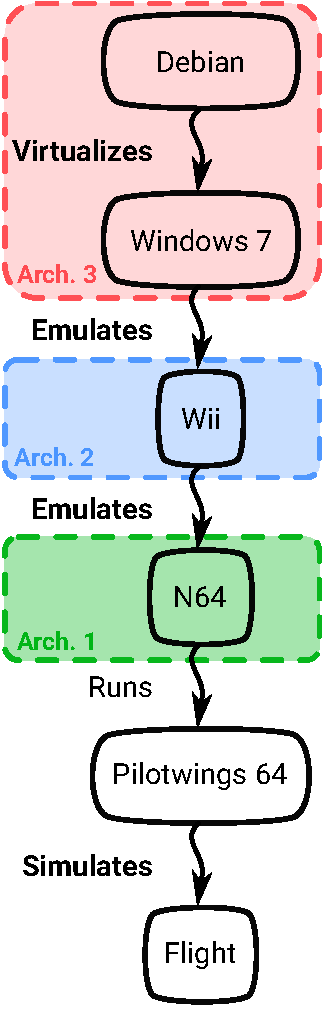
\includegraphics[width=.7\columnwidth]{../../img/arch_debian_win7_wii_n64_pw64_flight.pdf}
\end{center}
}
\end{column}
\end{columns}
\end{frame}
\begin{frame}[label={sec:org68c3c9a}]{OS-Level Virtualization}
\begin{center}
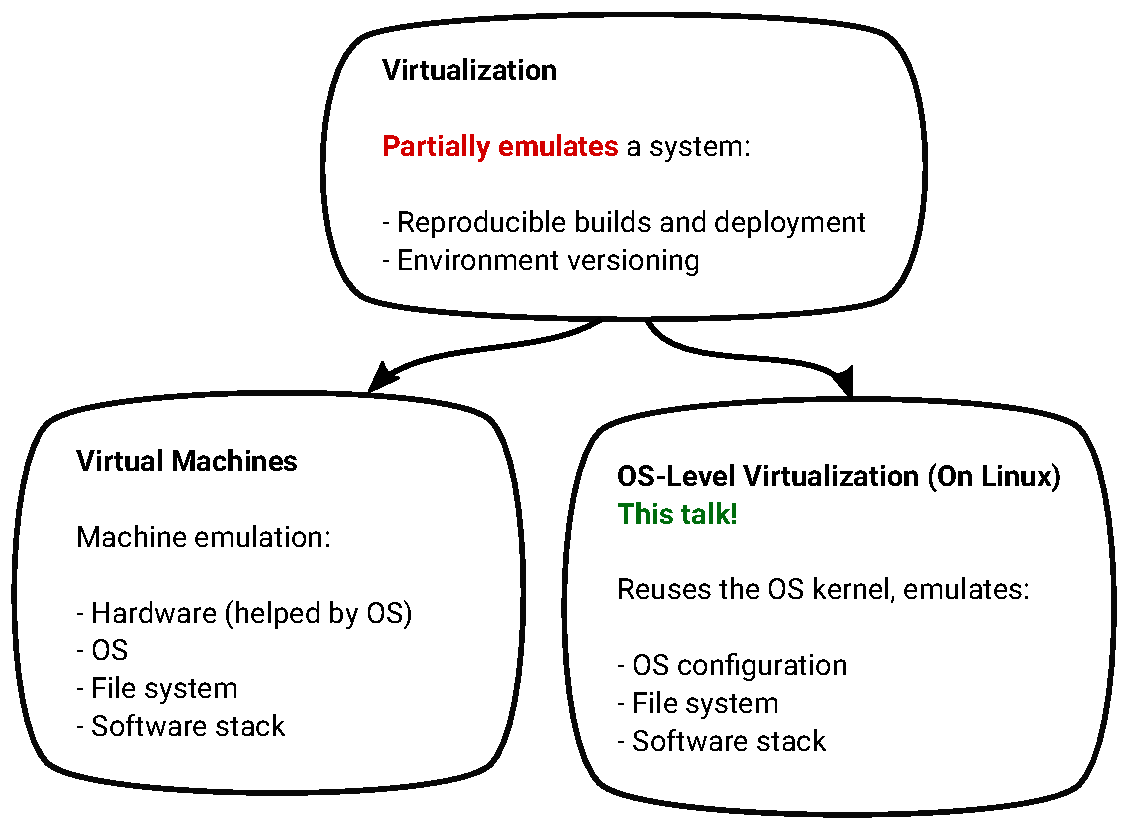
\includegraphics[width=.7\columnwidth]{../../img/virtualization_concept.pdf}
\end{center}
\end{frame}
\begin{frame}[label={sec:orge1ae3a5}]{OS-Level Virtualization on Linux}
\begin{center}
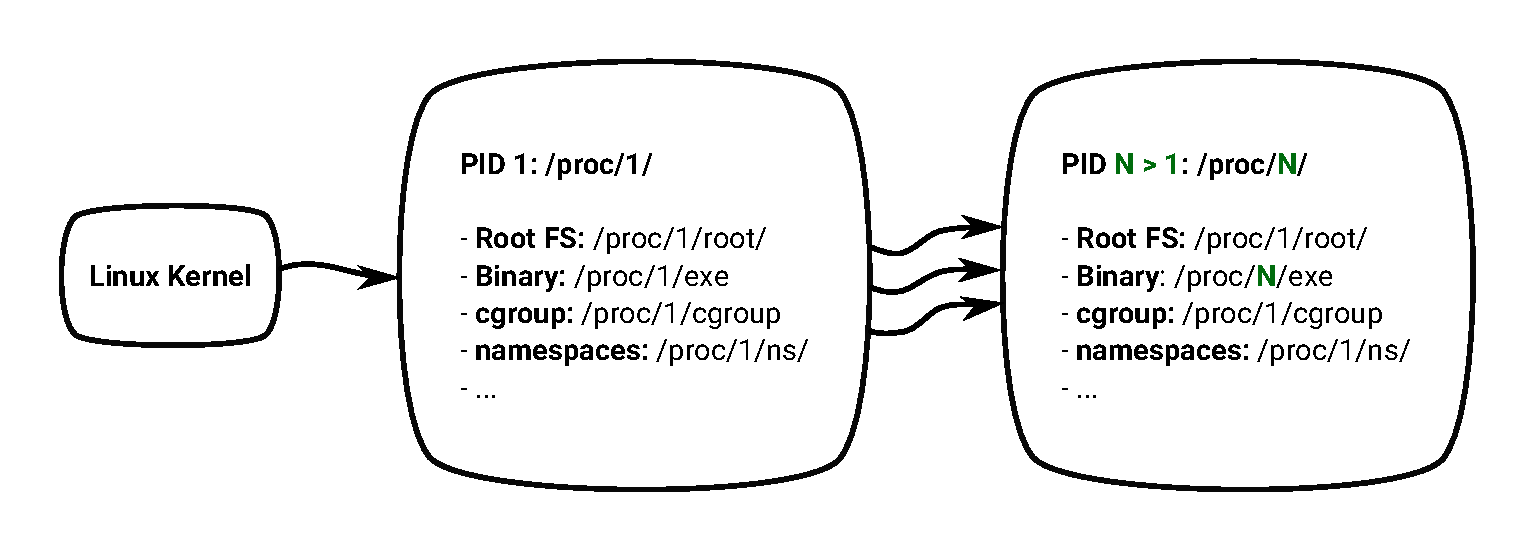
\includegraphics[width=\columnwidth]{../../img/virtualization_normal_kernel.pdf}
\end{center}
\end{frame}
\begin{frame}[label={sec:orgaddd8af}]{OS-Level Virtualization on Linux}
\begin{center}
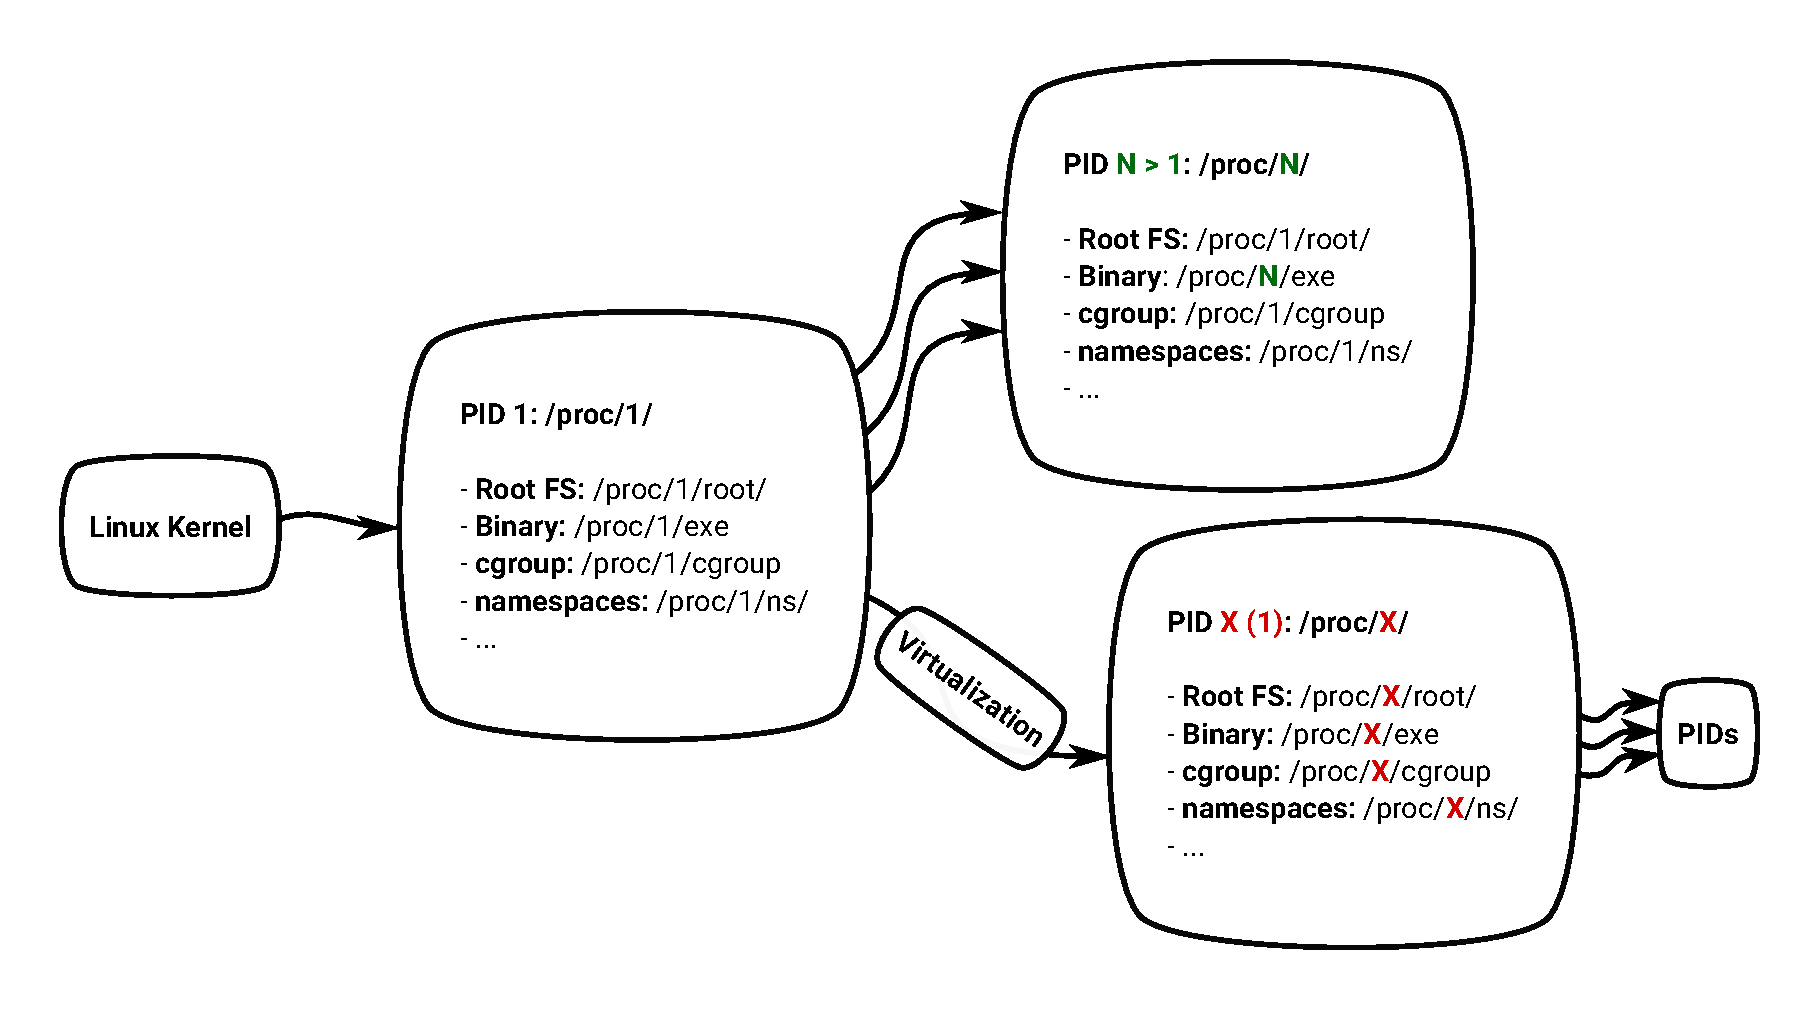
\includegraphics[width=\columnwidth]{../../img/virtualization_kernel.pdf}
\end{center}
\end{frame}
\section{Containers on Linux}
\label{sec:orgda21be7}
\begin{frame}[label={sec:org911e8ac}]{How Containers Work Zine}
Images used \alert{with permission}:
\begin{center}
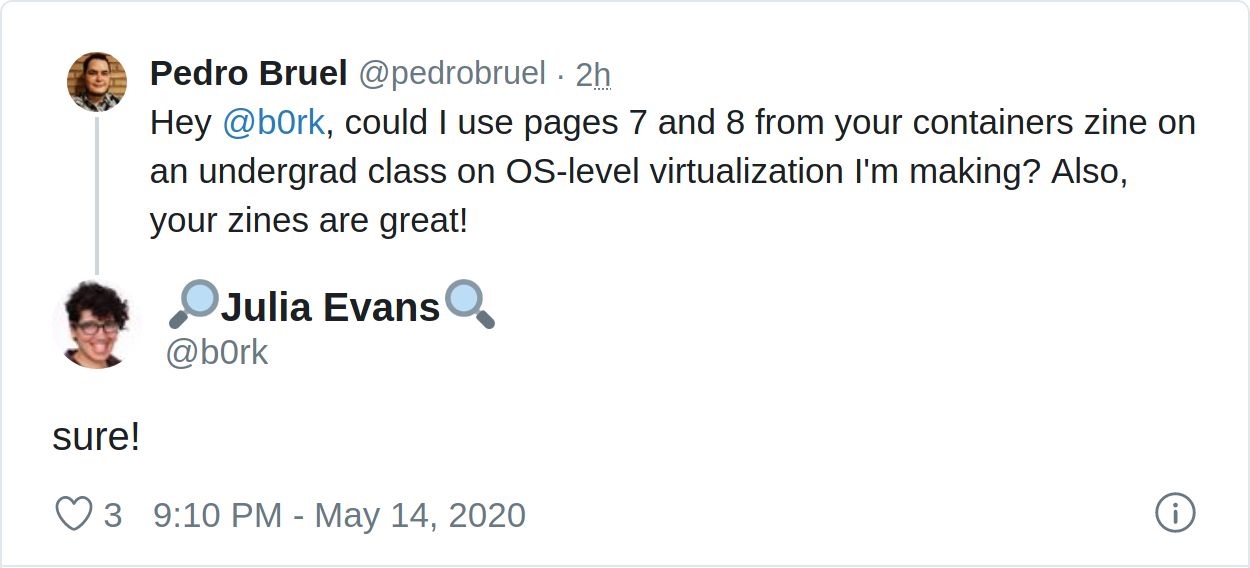
\includegraphics[width=.72\columnwidth]{../../img/hcw_permission_twitter.png}
\end{center}
\end{frame}
\begin{frame}[label={sec:org7be6430}]{Containers on Linux are Just Processes}
\begin{center}
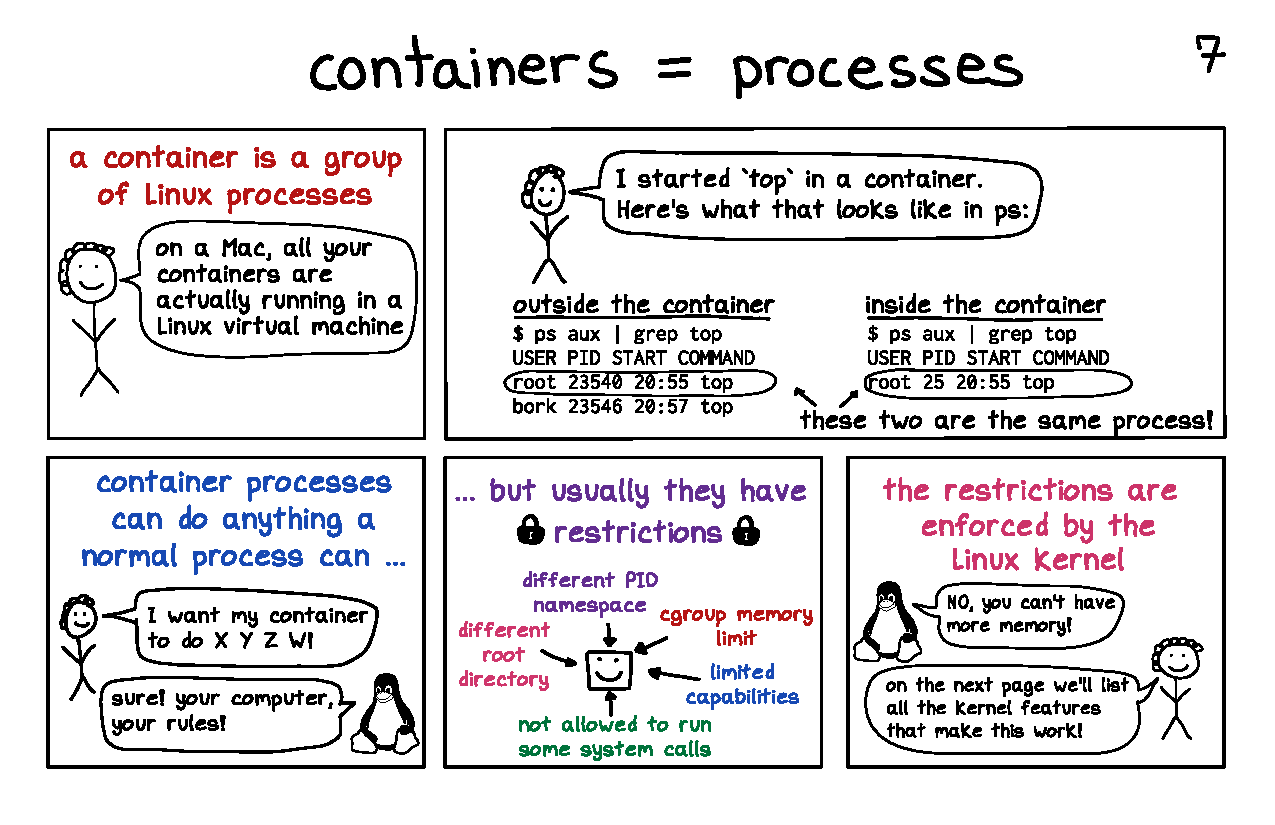
\includegraphics[width=.86\columnwidth]{../../img/how-containers-work_pg7.pdf}
\end{center}
\end{frame}
\begin{frame}[label={sec:org4de3152}]{Containers on Linux use Some Kernel Features}
\begin{center}
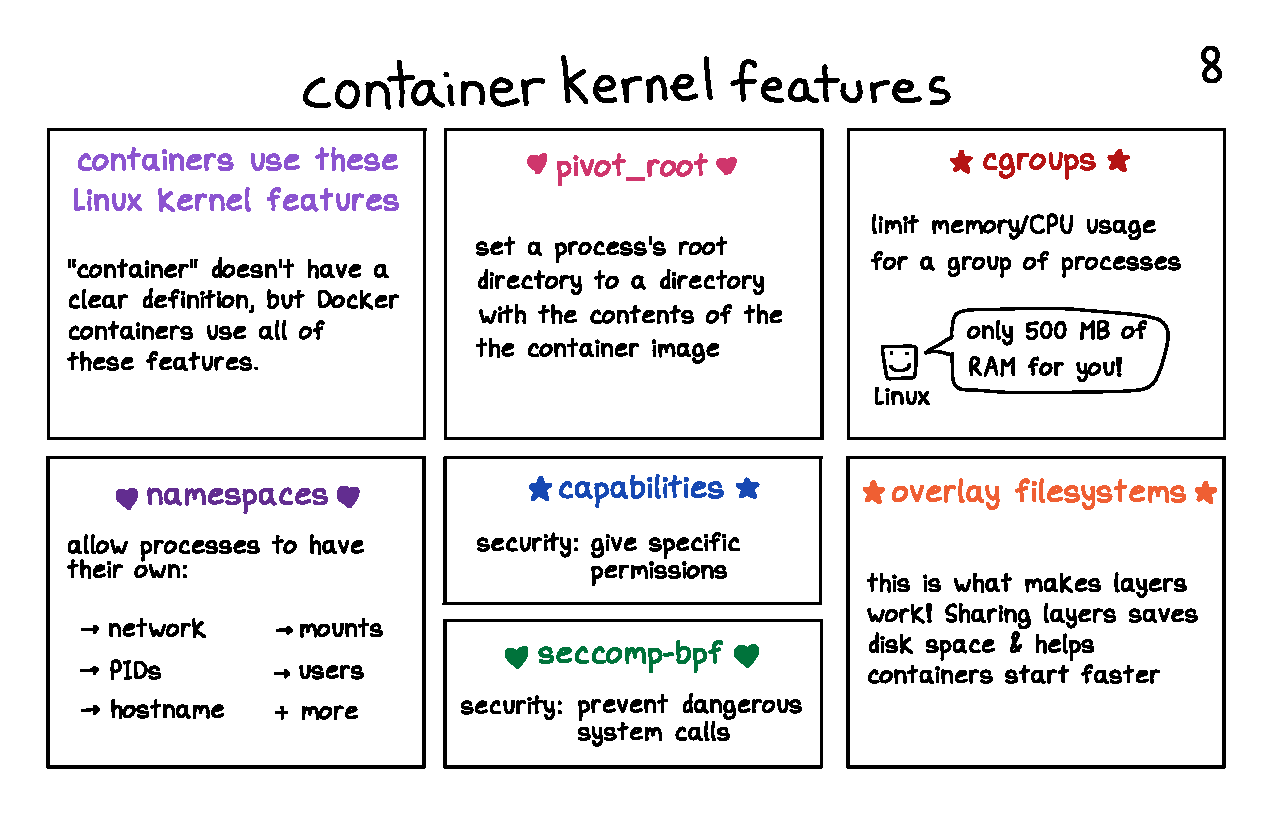
\includegraphics[width=.86\columnwidth]{../../img/how-containers-work_pg8.pdf}
\end{center}
\end{frame}
\section{Containers from Scratch}
\label{sec:org7c5b834}
\begin{frame}[label={sec:orgec764f8},fragile]{Containers from Scratch: Obtaing an Image}
 \lstset{language=bash,label= ,caption= ,captionpos=b,numbers=none}
\begin{lstlisting}
IMG_DIR="alpine_img"
IMG_URL="https://us.images.linuxcontainers.org/images/alpine/3.11/amd64/default/20200521_13:00/rootfs.tar.xz"
mkdir -p $IMG_DIR && curl $IMG_URL | tar xJ -C $IMG_DIR
\end{lstlisting}
\end{frame}
\begin{frame}[label={sec:org76a9658},fragile]{Containers from Scratch: Creating cgroups and Setting Limits}
 \lstset{language=bash,label= ,caption= ,captionpos=b,numbers=none}
\begin{lstlisting}
CGROUP_ID="MAC0475-145"
sudo cgcreate -g "cpu,cpuacct,memory:$CGROUP_ID"
sudo cgset -r cpu.shares=512 "$CGROUP_ID" # 1024 is 100% CPU
sudo cgset -r memory.limit_in_bytes=10000000000 "$CGROUP_ID"
\end{lstlisting}
\end{frame}

\section{Docker Containers}
\label{sec:orgca365b8}
\section{Docker Compose}
\label{sec:orgf4bae41}
\end{document}
